Największym wyzwaniem dla wydajności systemu okazało się generowanie opisów przez modele \gls{LLM}. Początkowa wersja kodu zakładała przetwarzanie wierszy pojedynczo: program tworzył wiersz, wysyłał zapytanie do serwera Ollama, czekał na odpowiedź i dopiero wtedy przechodził do kolejnego rekordu.

Pomiary wykazały, że wygenerowanie 100 recenzji produktów przez model Llama 3 zajmowało blisko 130 sekund. Prawie 95\% tego czasu stanowiło oczekiwanie na odpowiedź sztucznej inteligencji, podczas gdy zwykłe dane tekstowe (np. nazwiska z biblioteki Faker) generowały się w ułamki sekund. Czas oczekiwania na jeden rekord wynosił około 1,3 sekundy, a procesor oraz karta graficzna przez większość tego czasu nie były w pełni obciążone.

\subsection*{Algorytm dwufazowy i przetwarzanie wsadowe}
W celu lepszego wykorzystania zasobów obliczeniowych wprowadzono algorytm dwufazowy:
\begin{enumerate}
    \item W pierwszej kolejności aplikacja generuje wszystkie standardowe wiersze dla tabeli, całkowicie pomijając kolumny LLM. Działa to natychmiastowo i tworzy gotowe obiekty, które mogą posłużyć jako kontekst dla zapytań AI.
    \item Zebrane konteksty są następnie przekazywane w paczkach do oddzielnej funkcji, która zajmuje się wyłącznie komunikacją z modelem.
\end{enumerate}

Kluczem do przyspieszenia procesu okazało się grupowanie zapytań w mniejsze pakiety. Zamiast wysyłać pojedynczy wiersz, program opiera się na parametrze \texttt{SUB\_BATCH\_SIZE} (domyślnie 15) i wysyła do modelu kilkanaście kontekstów w jednym dużym prompcie. W odpowiedzi model zwraca tekstową strukturę \gls{JSON} zawierającą od razu cały pakiet wyników, co skraca narzut czasu potrzebny na wielokrotne inicjalizowanie zapytań przez silnik AI.

Dodatkowo zastosowano mechanizm \texttt{asyncio.Semaphore}, który zezwala serwerowi Ollama na przetwarzanie kilku takich paczek jednocześnie (domyślnie 8 zapytań w tle). Jeśli wystąpi błąd formatowania dla danej paczki (np. model pominie znak w odpowiedzi \gls{JSON}), uszkodzony fragment jest wyłapywany i przerabiany bezpiecznym, pojedynczym zapytaniem, aby nie psuć całego postępu generowania.

\subsection*{Dobór parametrów optymalizacji}
W celu dobrania optymalnych parametrów przeprowadzono pięć pomiarów na stałej próbce 100 wierszy z polami generowanymi przez \gls{LLM}. Każda próba dotyczyła innego sposobu wysyłania zapytań do modelu. Pomiary wykonano na laptopie z kartą NVIDIA RTX 5060, z modelem Llama 3 w Ollama --- ten sam sprzęt i ta sama próbka we wszystkich wierszach tabeli.

\begin{table}[H]
    \centering
    \begin{tabular}{|c|c|p{7cm}|}
        \hline
        \textbf{Próba optymalizacji} & \textbf{Czas [s]} & \textbf{Sposób generowania}                              \\
        \hline
        1                            & 129,52            & Jeden wiersz na raz --- wersja początkowa                \\
        \hline
        2                            & 218,88            & Wiele równoległych zapytań, ale nadal po jednym wierszu  \\
        \hline
        3                            & 63,43             & Kilka wierszy łączonych w jedno zapytanie (pakietowanie) \\
        \hline
        4                            & 124,41            & Pakietowanie z niekorzystnymi rozmiarami paczek          \\
        \hline
        5                            & 52,24             & Pakietowanie po 15 wierszy, maksymalnie 8 zapytań naraz  \\
        \hline
    \end{tabular}
    \caption{Porównanie wariantów generowania 100 wierszy AI (Ollama, RTX 5060)}
    \label{tab:llm_optimization_100}
\end{table}

Tabela \ref{tab:llm_optimization_100} pokazuje, że sama równoległość (próba 2) bez grupowania wierszy pogarsza wynik --- serwer Ollama zostaje przeciążony i czas rośnie do 219 s. Dopiero połączenie wielu wierszy w jednym prompcie (próba 3) skraca czas do około 63 s. Próba 4 potwierdza, że rozmiar paczki ma znaczenie: przy złych ustawieniach czas wraca do poziomu wersji sekwencyjnej. Wariant docelowy (próba 5) łączy pakietowanie z umiarkowaną równoległością i daje około 52 s --- blisko 2,5-krotnie szybciej niż wersja początkowa.

\subsection*{Wpływ rozmiaru paczki na czas generowania}
Aby precyzyjnie ocenić, jak liczba wierszy łączonych w jednym zapytaniu wpływa na wydajność, przeprowadzono dodatkową serię pomiarów. Wygenerowano 100 rekordów z polem tekstowym obsługiwanym przez \gls{LLM}, zmieniając wyłącznie parametr \texttt{SUB\_BATCH\_SIZE} (1, 2, 5, 10, 20 i 100). We wszystkich próbach utrzymano \texttt{MAX\_CONCURRENT=1}, tak aby wynik zależał głównie od wielkości paczki, a nie od równoległości zapytań. Testy wykonano z wykorzystaniem chmurowego API OpenAI (zamiast lokalnej instancji Ollama), co pozwoliło sprawdzić zachowanie modelu w warunkach zbliżonych do typowego wdrożenia produkcyjnego.

\begin{table}[H]
    \centering
    \begin{tabular}{|c|c|c|}
        \hline
        \textbf{Rozmiar paczki} & \textbf{Czas [s]} & \textbf{Uwagi}                                                 \\
        \hline
        1                       & 90                & generowanie pojedyncze --- punkt odniesienia                   \\
        \hline
        2                       & 60                & widoczne przyspieszenie dzięki mniejszej liczbie zapytań       \\
        \hline
        5                       & 43                & dalszy spadek czasu                                            \\
        \hline
        10                      & 30                & najkrótszy czas --- optymalny zakres dla testowanego modelu    \\
        \hline
        20                      & 76                & model zwracał niepoprawną liczbę wierszy; częsty fallback      \\
        \hline
        100                     & 121               & jedna paczka na całą próbkę; model ,,gubił'' format odpowiedzi \\
        \hline
    \end{tabular}
    \caption{Czas generowania 100 wierszy LLM przy różnych rozmiarach paczki (OpenAI API, MAX\_CONCURRENT=1)}
    \label{tab:batch_size_comparison}
\end{table}

\begin{figure}[H]
    \centering
    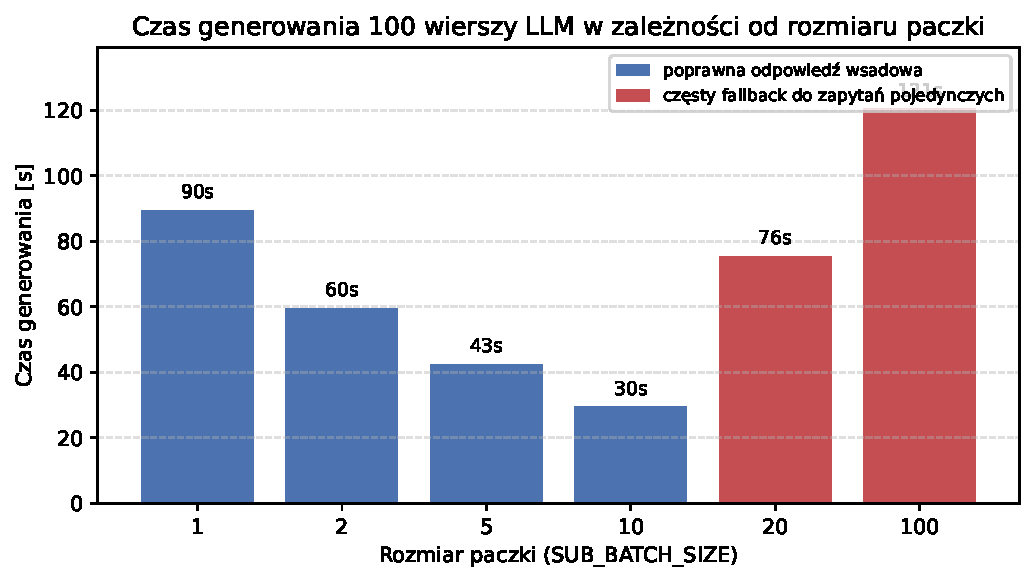
\includegraphics[width=0.85\textwidth]{images/batch_size_chart.pdf}
    \caption{Czas generowania 100 wierszy LLM w zależności od rozmiaru paczki}
    \label{fig:batch_size_chart}
\end{figure}

Wyniki zestawione w Tabeli \ref{tab:batch_size_comparison} i na Rysunku \ref{fig:batch_size_chart} pokazują wyraźną zależność: im więcej wierszy mieści się w jednym zapytaniu, tym krótszy jest łączny czas --- ale tylko do pewnej granicy. Przejście z paczki 1 na 10 skróciło generowanie z 90 s do 30 s, czyli około 3-krotnie. Każde kolejne zapytanie API niesie ze sobą narzut sieciowy i czas oczekiwania na odpowiedź modelu; grupowanie wierszy redukuje liczbę takich wywołań i dlatego daje realne przyspieszenie.

Od paczki 20 w górę trend się odwraca. Przy zbyt dużej liczbie wierszy w jednym prompcie model zaczął zwracać tablice \gls{JSON} o niepoprawnej długości -- zamiast dokładnie $N$ elementów otrzymywano krótsze lub dłuższe odpowiedzi. Silnik wykrywa ten błąd (porównanie \texttt{len(parsed\_array)} z oczekiwaną liczbą wierszy w paczce) i uruchamia mechanizm \textit{fallback}: uszkodzona paczka jest przerabiana ponownie, tym razem po jednym wierszu na zapytanie. Przy paczce 20 i 100 fallback uruchamiał się tak często, że łączny czas wzrósł do 76 s i 121 s --- wartości gorszych niż przy mniejszych, stabilnych paczkach.

Analiza wskazuje na dwa istotne wnioski. Po pierwsze, grupowanie wierszy w paczki skraca łączny czas generowania w porównaniu z wysyłaniem pojedynczych rekordów --- wariant sekwencyjny (\texttt{SUB\_BATCH\_SIZE=1}) okazał się najwolniejszy. Po drugie, zwiększanie rozmiaru paczki nie prowadzi monotonicznie do poprawy wydajności: przy zbyt dużych wartościach rośnie liczba błędów formatowania odpowiedzi, co wymusza kosztowny mechanizm \textit{fallback}. Dla testowanego modelu udostępnianego przez API OpenAI najkorzystniejszy czas uzyskano przy \texttt{SUB\_BATCH\_SIZE} równym 10; zakres 5--10 wierszy na zapytanie stanowi kompromis między liczbą wywołań API a stabilnością odpowiedzi. Wartość \texttt{SUB\_BATCH\_SIZE=15} zastosowana przy lokalnym serwerze Ollama (Tabela \ref{tab:llm_optimization_100}) została ustalona w odrębnych pomiarach --- potwierdza to, że optymalny rozmiar paczki zależy od dostawcy modelu i wymaga weryfikacji empirycznej w docelowym środowisku uruchomieniowym.

\subsection*{Porównanie wydajności Faker i LLM}
Kolejne pomiary wykonano na tym samym sprzęcie. Wykorzystano czterotabelowy schemat testowy \texttt{ecommerce\_llm\_\allowbreak schema}, w tym tabelę recenzji z polem \texttt{review\_text} generowanym przez \gls{LLM}.

\begin{table}[H]
    \centering
    \begin{tabular}{|l|c|c|c|}
        \hline
        \textbf{Typ danych}       & \textbf{Liczba wierszy} & \textbf{Czas (Faker)} & \textbf{Czas (\gls{LLM})}   \\
        \hline
        Proste (imię, adres)      & 1\,000                  & 0,8s                  & --                          \\
        \hline
        Proste                    & 10\,000                 & 5,2s                  & --                          \\
        \hline
        Złożone (z kontekstem AI) & 100                     & --                    & 52,24s (po optymalizacji)   \\
        \hline
        Złożone (z kontekstem AI) & 10\,000                 & --                    & 8\,038s ($\approx$2h 14min) \\
        \hline
    \end{tabular}
    \caption{Zestawienie czasów generowania danych strukturalnych i kontekstowych}
    \label{tab:performance_tests}
\end{table}

Jak widać w Tabeli \ref{tab:performance_tests}, generowanie danych przy użyciu algorytmów pseudolosowych (Faker) jest niezwykle szybkie i skalowalne liniowo. Wąskim gardłem systemu pozostaje generowanie treści przez \gls{LLM}, co potwierdza słuszność decyzji o zastosowaniu przetwarzania wsadowego z kontrolą współbieżności.

\subsection*{Alternatywny silnik --- vLLM}
Początkowe prace nad aplikacją oraz testy lokalne opierały się na serwerze Ollama \cite{ollama} --- narzędziu zaprojektowanym z myślą o prostocie obsługi i łatwym uruchamianiu modeli LLM na komputerach osobistych. Ollama wyróżnia się intuicyjnym interfejsem i prostym procesem instalacji, co doskonale sprawdza się przy deweloperskich eksperymentach. Jednakże w zastosowaniach chmurowych, wymagających dużej przepustowości i serwowania wielu równoczesnych zapytań, jego architektura nie oferuje optymalnej wydajności.

W celu maksymalizacji prędkości generowania w środowisku chmurowym przeprowadzono testy z wykorzystaniem vLLM \cite{vllm} --- biblioteki serwującej modele LLM, opracowanej na Uniwersytecie Kalifornijskim w Berkeley. vLLM różni się od Ollama podejściem architektonicznym: zamiast interfejsu zorientowanego na użytkownika końcowego, oferuje zaawansowany silnik zoptymalizowany pod kątem produkcyjnej wydajności i maksymalnego wykorzystania sprzętu.

Kluczowym mechanizmem vLLM jest \textit{PagedAttention} --- algorytm zarządzania pamięcią GPU inspirowany mechanizmami stronicowania pamięci z systemów operacyjnych. Standardowe podejście do obsługi mechanizmu uwagi \cite{attention_ml} w modelach LLM wymaga alokacji ciągłego bloku pamięci dla każdego zapytania, co prowadzi do fragmentacji i marnotrawstwa zasobów GPU. PagedAttention dzieli pamięć kontekstu KV-cache na małe, nieciągłe bloki, które mogą być dynamicznie przydzielane i zwalniane. Drugą istotną zaletą jest mechanizm \textit{continuous batching}, który dynamicznie łączy napływające zapytania w czasie rzeczywistym, bez konieczności czekania na skompletowanie całej paczki.

\subsubsection*{Konfiguracja vLLM na platformie Kaggle}
Wdrożenie vLLM w środowisku Kaggle wymagało rozwiązania dodatkowych problemów środowiskowych. Domyślna wersja vLLM (0.17) korzysta z biblioteki FlashInfer, która wymaga kompilacji kerneli CUDA w czasie wykonywania programu. System plików Kaggle, będący w dużej części środowiskiem tylko do odczytu, uniemożliwiał tę kompilację, powodując błędy budowania oprogramowania.

Rozwiązaniem okazało się zastosowanie starszej wersji vLLM (0.6.6), która zamiast FlashInfer wykorzystuje bibliotekę xFormers \cite{xformers}. xFormers dostarcza prekompilowane, wydajne implementacje operacji uwagi, co eliminuje konieczność kompilacji kerneli CUDA w czasie uruchamiania serwera.

Model Llama 3 8B-Instruct uruchomiono z podziałem tensorów na dwie karty Tesla T4 (\texttt{tensor-parallel-size=2}), co pozwoliło na wykorzystanie łącznie 32 GB pamięci VRAM. Aplikacja, dzięki oparciu komunikacji na standardzie OpenAI API, wymagała jedynie zmiany adresu URL serwera modelu oraz wyłączenia sztucznego podziału na paczki --- dotychczasowy interfejs i logika przetwarzania po stronie backendu pozostały niezmienione, delegując pełne zarządzanie ruchem do silnika vLLM.

\subsection*{Skalowalność dla dużych zbiorów danych}
W celu ostatecznego porównania wydajności wykonano próbę obciążeniową polegającą na wygenerowaniu bazy danych zawierającej 10\,000 wierszy przetworzonych przez \gls{LLM}. Testy przeprowadzono na dwóch platformach sprzętowych oraz z dwoma silnikami inferencji (Ollama i vLLM).

\begin{table}[H]
    \centering
    \begin{tabular}{|l|l|c|c|c|}
        \hline
        \textbf{Środowisko testowe} & \textbf{Silnik} & \textbf{Wierszy AI} & \textbf{Czas [s]} & \textbf{Czas/wiersz [s]} \\
        \hline
        Laptop (RTX 5060)           & Ollama          & 100                 & 52,24             & 0,52                     \\
        \hline
        Laptop (RTX 5060)           & Ollama          & 10\,000             & 8\,038,12         & 0,80                     \\
        \hline
        Kaggle (2x Tesla T4)        & Ollama          & 100                 & 178,02            & 1,78                     \\
        \hline
        Kaggle (2x Tesla T4)        & Ollama          & 10\,000             & 14\,860,23        & 1,49                     \\
        \hline
        Kaggle (2x Tesla T4)        & vLLM            & 100                 & 18,30             & 0,18                     \\
        \hline
        Kaggle (2x Tesla T4)        & vLLM            & 10\,000             & 1\,693,50         & 0,17                     \\
        \hline
    \end{tabular}
    \caption{Porównanie skalowalności w zależności od sprzętu i silnika}
    \label{tab:llm_scalability}
\end{table}

\begin{figure}[H]
    \centering
    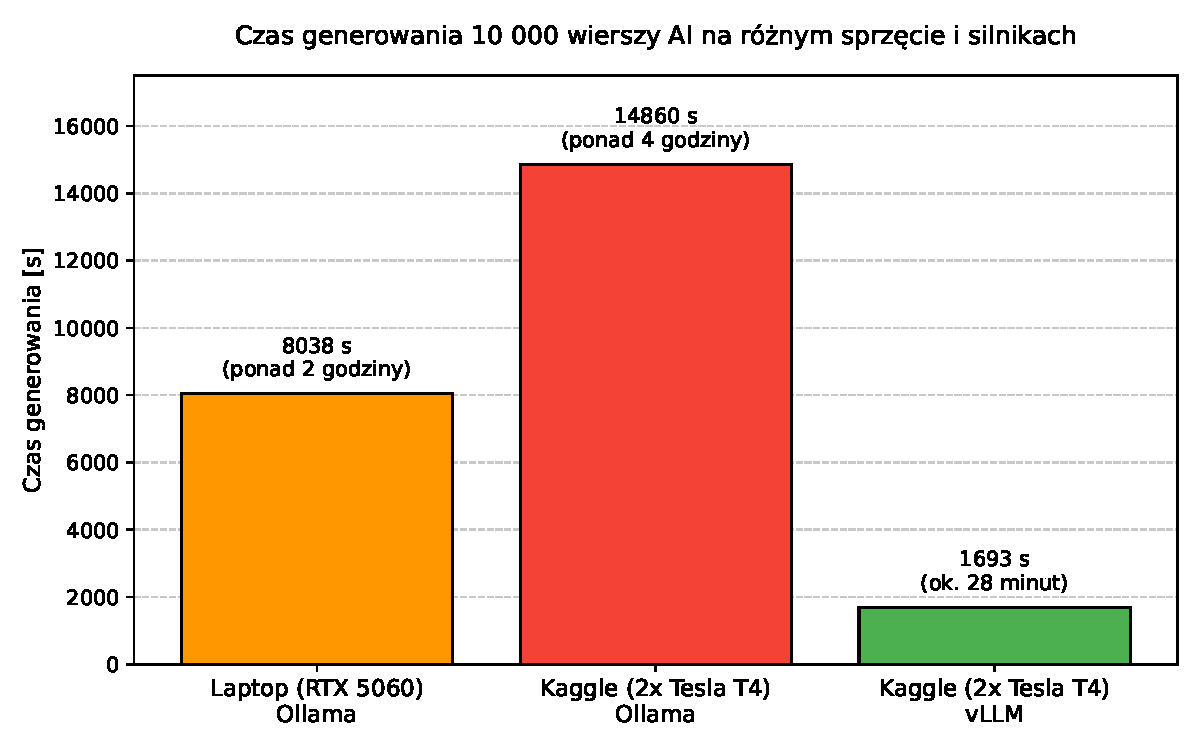
\includegraphics[width=0.85\textwidth]{images/hardware_comparison_chart.pdf}
    \caption{Wykres porównujący czas generowania 10\,000 wierszy AI na różnym sprzęcie}
    \label{fig:hardware_chart}
\end{figure}

Jak przedstawia Rysunek \ref{fig:hardware_chart}, wygenerowanie 10\,000 wierszy na laptopie z serwerem Ollama zajęło ponad 8\,038 sekund (nieco ponad 2 godziny). Długotrwałe obciążenie karty graficznej wiązało się ze zjawiskiem tzw. \textit{thermal throttling} (zabezpieczenie przed przegrzaniem obniżające taktowanie procesora), przez co średni czas utworzenia jednego wiersza wzrósł z 0,52 do 0,80 sekundy. Mimo to aplikacja zniosła ten test poprawnie i zapisała całą tabelę w pliku bazy SQLite.

Dla porównania, ten sam schemat z serwerem Ollama uruchomiono w darmowym środowisku chmurowym Kaggle, dysponującym dwoma kartami Tesla T4 (łącznie 32 GB pamięci VRAM). Pełna próba 10\,000 wierszy na Kaggle zajęła aż 14\,860 sekund (ponad 4 godziny). Różnica wydajności względem laptopa wynika ze specyfikacji sprzętowych --- karty Tesla T4 oparte są na architekturze Turing \cite{turing_microarchitecture} z 2018 roku, która nie posiada ulepszonych jednostek obliczeniowych obecnych w nowoczesnych kartach z serii RTX (architektura Ada Lovelace \cite{ada_lovelace_microarchitecture}).

Zastąpienie serwera Ollama przez vLLM na tej samej platformie Kaggle przyniosło drastyczną poprawę wydajności. Generowanie 100 wierszy AI skróciło się ze 178 do zaledwie 18,3 sekundy (przyspieszenie blisko 10-krotne), a pełna próba 10\,000 wierszy ze 14\,860 do 1\,693 sekund (około 28 minut zamiast ponad 4 godzin) --- przyspieszenie blisko 9-krotne. Średni czas na wiersz z vLLM (0,17 s) okazał się ponad 4-krotnie lepszy niż najlepsza lokalna konfiguracja Ollama na laptopie RTX 5060 (0,52 s). Wynik ten potwierdza, że mechanizmy PagedAttention i \textit{continuous batching} zaimplementowane w vLLM pozwalają na znacznie efektywniejsze wykorzystanie chmurowych zasobów GPU niż tradycyjne podejście serwera Ollama.
